%This work is licensed under the Creative Commons Attribution-NonCommercial-NoDerivs 3.0 United States License. To view a copy of this license, visit http://creativecommons.org/licenses/by-nc-nd/3.0/us/ or send a letter to Creative Commons, 444 Castro Street, Suite 900, Mountain View, California, 94041, USA.

\section{Nanopatterned (Plasmonic) Photocathodes}

In the search for alternative mechanisms to reduce the intrinsic divergence of the electron beam upon photoemission, a possible area of interest was Plasmon-Assisted Photoemission (PAPE). 
As the name suggests, a plasmon is the quasiparticle of plasma oscillation.
When this occurs at the surface of a conducting material, the resultant quasiparticles are called ``surface plasmon-polaritons.''
Since these will be the only plasmons discussed in this thesis, the word ``plasmon'' will be used interchangeably for the name ``surface plasmon-polariton.''
Electrons in a conductor can couple with electromagnetic fields, in this case a laser field, and oscillate accordingly.
This overall oscillation of electrons near the surface of the conductor creates strong oscillatory local surface electric field~\cite{cottam_introduction_2004,concepts_2002}.
In PAPE, the goal is use this field to both enhance the emission and `control' the divergence of photoemitted electrons through the combined action of photoemission barrier suppression and ponderomotive acceleration.
On the other hand, these oscillating electrons are nothing but an oscillating current, and thus if a large plasmon response is established, resistive heating is a major concern even for the small resistivities typical of conductors.

This avenue of investigation was motivated by Zawadzka et al~\cite{zawadzka_evanescent_2001} who indicate that when driving a surface plasmon on gold they witnessed a reduction in the emission angle of photoemitted electrons.
In their paper, the authors coat a thin gold film on a prism; the laser then ``back illuminates'' the gold through the prism, ejecting electrons on vacuum side of the foil.
This arrangement is called the Kretschmann geometry.
While this geometry is common, due to fears about the lack of heat conduction through the glass and the power needed to generate a sufficient electron beam current, we felt that for UEM applications we should explore the alternative ``grating coupling'' geometry~\cite{kupersztych_ponderomotive_2001,kupersztych_anomalous_2005,li_surface_2013}.
In this geometry, the plasmon is driven on a periodic surface rather than a flat surface attached to glass.
Further, in this front-side illuminated geometry the back surface is now free to be attached to a heat sink.

\subsection{The Grating Coupling Geometry}

Every conducting material has an intrinsic plasma frequency given by 
\begin{equation}
  \omega_{P} = \sqrt{\frac{\rho_{e} e^2}{\varepsilon_{0} m^*}} \,\text{,}
\end{equation}
where $\rho_{e}$ is the free-electron density and $m^*$ is the electron effective mass in the material.
And in the most simple (undamped) approximations, $\varepsilon$, the real part of the dielectric function of the material, may be written in the following form:
\begin{equation} \label{eq:dielectric_as_omega}
  \varepsilon(\omega) = 1 - \frac{ \omega_{P}^2 }{ \omega^2 } \,\text{.}
\end{equation}

At the interface of a vacuum and such a simple material, constraints on the material parameters which may allow surface plasmons, result in the condition that the dielectric constant at the oscillation frequency of the surface plasmon $ \varepsilon(\omega_{SP}) = -1 $~\cite{cottam_introduction_2004}.
Substituting this result into \ref{eq:dielectric_as_omega} shows that this frequency of oscillation is simply related to intrinsic plasma frequency by
\begin{equation}
  \omega_{SP} = \omega_{P} / \sqrt{2} \,\text{.}
\end{equation}
Further, plasmons propagating along a vacuum interface carry momentum whose magnitude is given by 
\begin{equation}
  k_{SP}^2 = \frac{\omega^2}{c^2} \left( \frac{ \varepsilon }{ 1 + \varepsilon } \right) \,\text{.}
\end{equation}

In the grating coupling scheme (shown in \ref{fig:plasmon_schematic}) a laser of wavelength $\lambda$ is incident on a material with a grating of period $d$, making an angle $\theta$ from the surface normal.
A surface plasmon is driven when the sum of the component of the laser wave-vector parallel to the material surface ($k_{Lx}$) and a Fourier component ($k_{G} = 2 \pi / d$) of the grating matches the wave-vector of the surface plasmon
\begin{equation}
  k_{SP} = k_{Lx} + n k_{G} \,\text{,}
\end{equation}
where $n$ here is an integer.
This expression reduces to 
\begin{equation} \label{eq:plasmon_condition}
  \sqrt{ \frac{ \varepsilon }{ 1 + \varepsilon } } = \sin \theta + \frac{ n \lambda }{ d } \,\text{,}
\end{equation}
where $\lambda$ is the incident laser wavelength.
For a given grating period, \ref{eq:plasmon_condition} determines the angle of incidence that the laser must make with the surface in order to drive the plasmon.
Alternatively, it may be used to design the periodic surface structure, for example allowing for angles that the microscope column will accept, different driving orders ($n$), and even other Fourier components of the periodic surface structure.

\begin{figure}
  \centering
  \begin{tikzpicture}

\draw [orange!70,fill=orange!30]
  (0,0)
  \foreach \x in {1,2,...,5}{
    -- ++(0.25, 0)
    -- ++(0, 0.25)
    -- ++(0.5, 0)
      coordinate [pos=0.5] (mid-\x)
    -- ++(0, -0.25)
    -- ++(0.25, 0)
  }
  -- ++(0,-1)
  -- ++(-5,0)
  -- cycle
;

\draw [dashed]
  (mid-3)
  -- ++(0,3)
    node [left=0.3, pos=0.4] {$\theta$}
;

\draw [green, thick,->]
  (0,3)
  -- (mid-3)
;
\draw [green, thick,->]
  (mid-3)
  -- (5,3)
;

\node at (0.5, -0.45) {$\varepsilon$};

\draw [thick, |-|]
  ($(mid-4)+(0,-0.7)$)
  -- ++ (1, 0)
    node [fill=orange!30, pos=0.5] {$d$}
;
  

\end{tikzpicture}

  \caption[Grating coupling geometry for driving a surface plasmon]{Schematic diagram of a grating coupling geometry for driving a surface plasmon}
  \label{fig:plasmon_schematic}
\end{figure}

\subsection{Commercial Grating on Glass}

For proof-of-concept purposes, the first experiment was performed on a commercially available gold foil on glass holographic grating (750 lines/mm).
Like the Kretschmann geometry, a foil on glass grating is vulnerable to heating problems; a plasmon creates a large amount of heat but the glass is a poor heat conductor.
The aforementioned laser (emitting $\sim$200fs pulses of green light at a peak pulse intensity of 30MW/cm$^2$) was used to drive the plasmon.

\begin{figure}
  \centering
  \begin{tikzpicture}
  \node{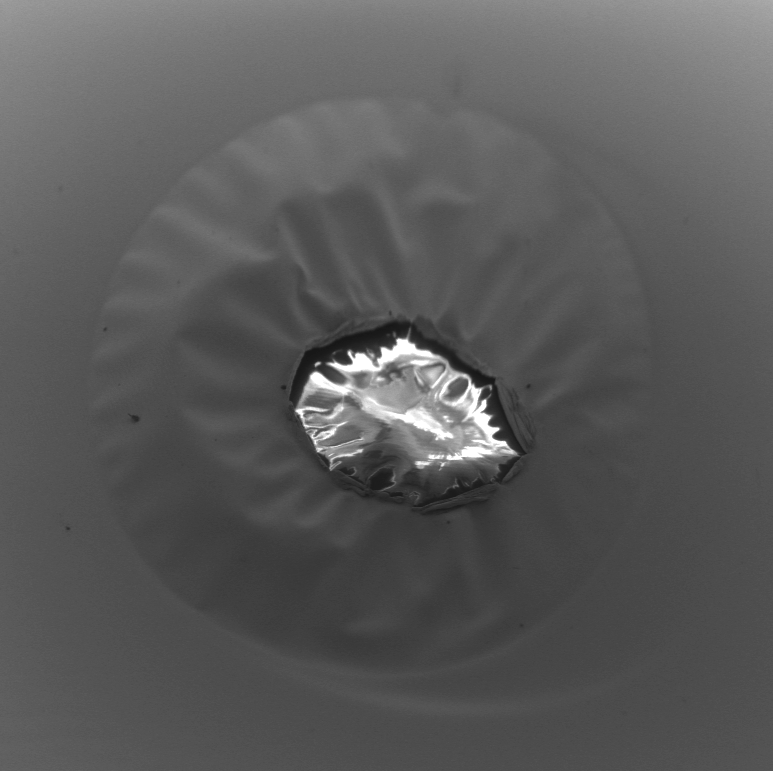
\includegraphics{damage.png}};
  \draw[|-|, thick] (-3.5,-3.5) -- ++(1.425,0) node [above,pos=0.5] {$0.2$mm};
  % full diameter of (well defined) damage spot is 0.8mm
\end{tikzpicture}

  \caption{Damage to commercial gold-on-glass holographic grating}
  \label{fig:grating-damage}
\end{figure}

The input laser angle was slowly changed until the plasmon oscillation is visible.
At the instant that the plasmon started, a bright flash was visible on the scintillator screen and then disappeared.
After this, the grating showed visual signs of damage, both on the surface and in the reflected light pattern.
\ref{fig:grating-damage} shows the results of Scanning Electron Microscopy (SEM) on the grating.
The damage pattern is round and of the size of the laser spot used to drive the plasmon.
The extent of the damage indicates a large temperature increase, which given the other evidence of the test, can be assumed to be from the sudden appearance of a surface plasmon.

There are several conclusions that can be drawn from this experiment.
Most importantly, it shows that a plasmon was driven successfully; given the angular dependence and large response, few other processes could have occurred.
The heat generated by the plasmon oscillation destroyed the grating, therefore it validated the decision not to pursue a Kretschmann geometry over fears of heat damage at the high heating rates of the laser-plasmon interaction.
Finally, it suggests that through the use of a thermally conductive and structurally sound photoemission material and mount for the plasmonic photocathode, PAPE might generate a large number of electrons (as evident by the bright flash).

\subsection{Sinusoidal Grating}

After the destruction of the gold foil on glass grating, new gratings were designed to have a higher substrate thermal conductivity.
The second generation grating was constructed from a silicon substrate then coated with a gold film.
The thermal conductivity of silicon is approximately 100 times that of glass. %TODO reference needed?

\begin{figure}
  \centering
  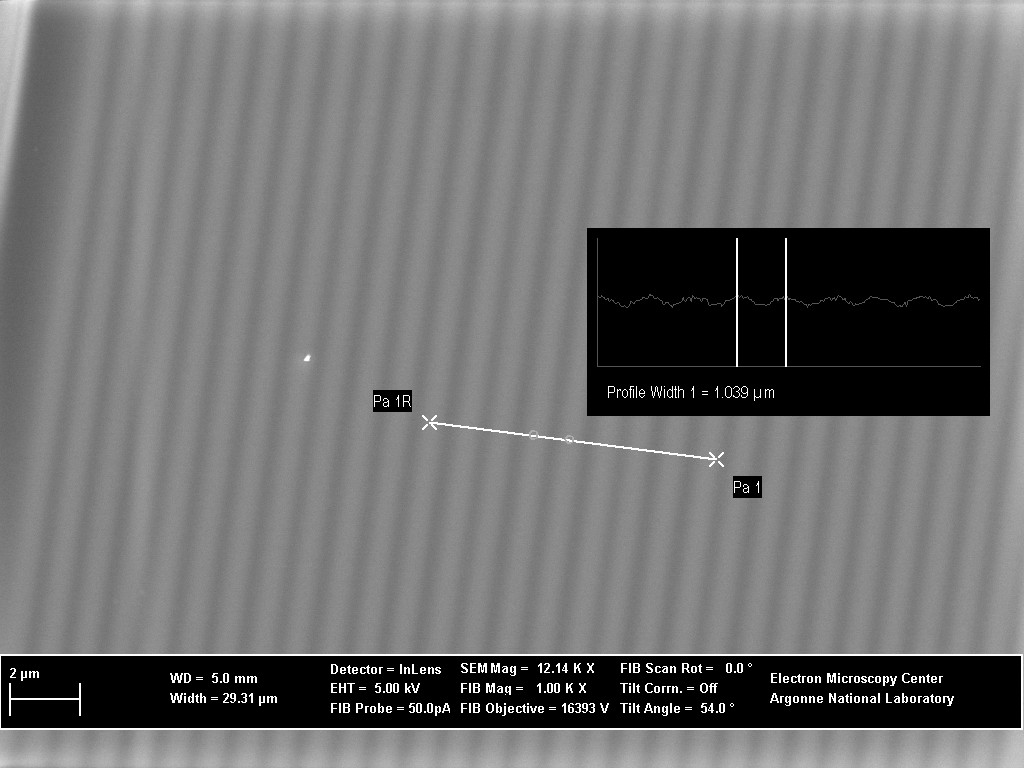
\includegraphics{HighMagSEM.jpg}
  \caption[SEM image of sinusoidal grating on silicon]{
    SEM image of sinusoidal grating on silicon.
    Pattern milled by focused ion beam milling at Argonne National Lab.
    Sample was later coated with 300 nm gold film.
  }
  \label{fig:fib-si-sem}
\end{figure}

Collaborators at Argonne National Laboratory's Electron Microscopy Center, Material Science Division employed a defocused Gallium focused ion beam (FIB) (Zeiss 1540XB) to mill an approximately sinusoidal shape into the surface of a silicon wafer.
Several regions were created each 100x100$\mu$m in area, having a $\sim$1$\mu$m period and $\sim$10\% modulation depth.
By \ref{eq:plasmon_condition}, given a laser wavelength of 523nm ($\varepsilon_{Au} \approx -3.95$~\cite{johnson_optical_1972}), this choice of periodicity corresponds to an incidence angle of $\sim39^{\circ}$, which is within the acceptance range of our experimental setup (35-75$^{\circ}$) (see Section \ref{sec:gun_design}).
An SEM image of one such region is shown in \ref{fig:fib-si-sem}.
A 300nm film of gold was deposited onto the silicon using the Varian e-beam deposition chamber at the UIC Nano Core Facility (NCF); a thin layer of chromium was deposited between the silicon and gold as a binding agent.
As the gold film is many times thicker than the penetration depth of green light on gold and several times thicker than the penetration depth of the plasmon field, neither the laser radiation nor the plasmon field will couple with the silicon.
%TODO should I comment on the coating acting to smooth the surface to a proper sinusoid?

\begin{figure}
  \centering
  \begin{tikzpicture}
  \inputdata{power_seq_data}
\end{tikzpicture}

  \caption[Photoemission characteristics of laser-driven plasmons on a one-dimensional periodic gold surface]{
    Photoemission characteristics of laser-driven plasmons on a one-dimensional periodic gold surface.
    Top: Electron emission strength as a function of incident 523nm femtosecond laser pulse intensity for coherently-driven plasmons (top curve)
      % with parabolic fit to initial dependence (dashed curve)
      and comparative emission from a plane gold surface under the same irradiation conditions.
    Bottom: Two-dimensional electron momentum distributions for plasmon-assisted emission (A-D) and two-photon field emission from gold (E) at the laser intensities indicated on the top graph.
    The circular aperture visible in B-D is the 6mm-diameter bore of the magnetic focusing lens.
    The orientation of the grating lines of the periodic gold surface with respect to the emission in A-D is parallel to the broadening seen in B-D.
  }
  \label{fig:pape}
\end{figure}

% Content taken from 2010 ANL report
\ref{fig:pape} summarizes the photoemission results obtained from this gold-coated periodic photocathode under green (523nm) laser irradiation.
Strong enhanced photoemission was observed for only a narrow $\pm$5mrad range of incidence angles $\theta$ around the expected plasmon resonance angle of 39$^{\circ}$.
Moreover, this enhanced laser-driven electron emission was only observed for $p$-polarized incident 523nm femtosecond laser radiation.
These two properties are known characteristics of plasmon-assisted photoemission~\cite{kupersztych_ponderomotive_2001,kupersztych_anomalous_2005,li_surface_2013}.

As seen in \ref{fig:pape}, at low incident laser intensities, below a laser intensity of about 25MW/cm$^2$, the emission from the nano-patterned photocathode at the plasmon resonance condition is very similar to that observed from a flat gold surface neighboring the FIB-milled region.
Specifically, the strength of both emissions have a quadratic dependence on the incident laser intensity.
This is consistent with a two-photon field emission process --- it requires the absorption of two 2.37eV (green) photons for an electron to acquire sufficient energy to allow any significant field emission as gold has a work function of $\sim$5eV.
Moreover, both emissions have similar momentum distributions (\ref{fig:pape} A and E), again indicating a similar emission process.
The only difference is that the emission from the nano-patterned region is 3-4 times more efficient.
This is readily explained by the fact that the periodic surface modulation results in a local enhancement of the $\sim$1MV/m DC gun field at the peaks of the modulation which, through the Schottky effect, then presents a reduced barrier for field emission.

I note here that for these measurements, the relative emission efficiencies are calculated from the integration of the luminosity detected on the YAG scintillator screen.
The scintillator and CCD camera detection scheme was shown to be linear (i.e., integrated signal proportional to number of electrons per pulse) for at least $10^4$ electrons per pulse, using the known linearity of single-photon photoemission from Ta irradiated by our 261nm ultraviolet laser source.
%TODO introduce this linearity earlier?
As a result, the detection scheme will accurately determine any laser power law dependence to the electron emission from the photocathode.

Above an incident laser pulse intensity of $\sim$32MW/cm$^2$, there is a rapid and dramatic increase in the emission efficiency for the nano-patterned photocathode.
This can be explained by a suppression of the barrier to photoemission below the two-photon excitation energy, thus allowing direct two-photon photoemission.
The well-known Schottky Effect states that for an applied electric field $E$ the work function will be suppressed by an amount
\begin{equation}
  \Delta \Phi = - e\sqrt{\frac{e E}{4 \pi \varepsilon_{\smallzero}}} \,\text{.}
\end{equation}
This suppression is likely caused by the laser-excited surface plasmon, since on the neighboring flat gold surface, where the suppression due to the laser (20MV/m) and the 20kV acceleration potential (0.8MV/m) is $\Delta \Phi \approx $ 0.18eV, no similar increase in efficiency is observed.
If this is indeed the case, and the surface plasmon field further suppresses the barrier to a total $ \Delta \Phi \approx $ 0.35eV to allow direct two-photon photoemission, the field must be of the order of 60MV/m or three times that of the laser field.
In \ref{fig:pape} B, at a laser intensity of $\sim$30MW/cm$^2$, there is already a distinct broadening of the momentum distribution in the direction parallel to the wavevector $k_G$ of the sinusoidal modulation on the photocathode (i.e., perpendicular to the FIB-milled grooves). 
This broadening becomes the dominant feature of the electron emission above $\sim$32MW/cm$^2$; indeed, it becomes so severe that at laser intensities above $\sim$37MW/cm$^2$ the 6mm-diameter bore of the magnetic lenses becomes a strong limiting aperture for the resulting beam --- as is clearly seen in \ref{fig:pape} D and by the cut-off in the detected electron signal (YAG fluorescence).

\subsection{Sinusoidal Grating, Rotated}

In principle, this unexpected increase in transverse momentum (\ref{fig:pape} B and C) could be caused by any of three effects.
The first, and most easily ruled out, is that the electric field of the laser itself could affect the electrons, causing the divergence.
The possibility is easily dismissed as the effect is not observed when off the grating.
The second possible cause is the divergence of the plasmon's own electric field ($\partial E_{plasmon} / \partial x$).
This field is parallel to the surface plasmon vector $k_{SP}$ (assumed here to be in the $x$ direction).
The third possible cause is local field enhancement of the accelerating electric field due to the peaks in the sinusoidal shape of the surface, commonly known as the ``lightning rod'' effect.
For the employed one dimensional grating, this effect is necessarily parallel to the grating vector $k_G$.

\begin{figure}
  \centering
  \begin{tikzpicture}
  \draw [thick,->,green] 
    (0,0) -- ++(3,0) 
      node [pos=0.5,below,black,align=center] {$k_L \sin \theta$\\$\theta \approx 39^{\circ}$}
  ;
  \draw [thick,->,blue]
    (3,0) -- ++(2,0)
      node [pos=0.5,below,black] {$k_G$}
  ;
  \draw [thick,->,red]
    (0,0.2) -- ++(5,0)
      node [pos=0.5,black,above] {$k_{SP}$}
  ;
  \node at (7,0) {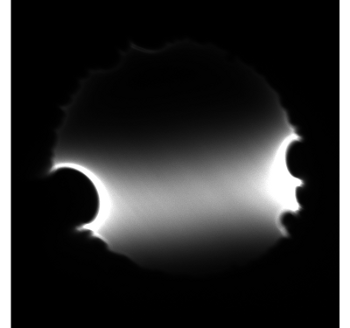
\includegraphics{final-fourier-030.png}};
  \draw [very thick,red] (6,-0.4) -- ++(9:2.2);

  \draw [thick,->,green] 
    (0,-3.5) -- ++(3,0) 
      node [pos=0.5,below,black,align=center] {$k_L \sin \theta$\\$\theta \approx 47^{\circ}$}
  ;
  \draw [thick,dashed,green] 
    (3,-3.5) -- (4,-3.5)
      node [above,black,pos=0.8] {$45^{\circ}$}
  ;
  \draw [thick,->,blue]
    (3,-3.5) -- ++(1.4,1.4)
      node [pos=0.2,above left,black] {$k_G$}
      coordinate [pos=1] (end)
  ;
  \draw [thick,->,red]
    (0,-3.5) -- (end)
      node [pos=0.5,black,above] {$k_{SP}$}
  ;
  \node at (7,-3) {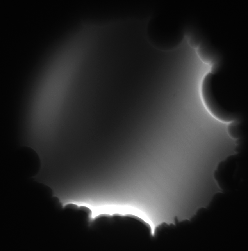
\includegraphics{rotated.png}};
  \draw [very thick,red,dashed] 
    (6,-2.7) -- ++(9:2.2)
      node [pos=0.7,below, white] {$45^{\circ}$}
      coordinate [pos=1] (rotate end)
  ;
  \draw [very thick,red]
    (rotate end) -- ++(234:2.2)
  ;
\end{tikzpicture}

  \caption[Comparison of the collinear and rotated plasmonic excitation geometries]{
    Comparison of the collinear (above) and rotated (below) plasmonic excitation geometries.
    This rotation separates the directionality of effects caused by the laser, plasmon field and grating.
    Each vector diagrams (left) is shown next to a representative observed momentum distribution image (right).
    The increased divergence is shown to be rotated by the same $45^{\circ}$ as the grating (the original collinear line is shown dashed); evidence that the grating is the cause of the deleterious effect.
  }
  \label{fig:rotated}
\end{figure}

Given the geometry of the previous measurement, notably the collinear arrangement of plasmon vector and the grating vector, the true cause is difficult to determine.
However, if instead the grating is rotated --- and the laser incidence angle is corrected to account for the longer effective periodicity of the surface --- the directionality of these effects may be separated.
The left side of \ref{fig:rotated} shows the comparison of the grating vector geometries for the original scheme (top) and one in which the grating is rotated by $45^{\circ}$ (bottom).
For this rotation, the laser angle must be increased from $39^{\circ}$ to $47^{\circ}$.

The experimental results are shown to the right in \ref{fig:rotated}.
As the divergence is clearly shown to be rotated by $45^{\circ}$ with respect to the collinear case, this experiment demonstrates that the cause of the divergence increase is due to the local field enhancements near the peaks of the grating.
For a mathematical treatment of the transverse electric field of such patterned surfaces, the reader is referred to Ref.~\cite{watts_sharp_1997}. 
Our results are commensurate with the results shown by Zawadzka et al~\cite{zawadzka_evanescent_2001}, who showed a reduced divergence in the Kretschmann geometry.
As that geometry does not employ a patterned surface, it would not be subject to such local field enhancements of the accelerating electric field.


\subsection{Trenched Grating}

In an attempt to mitigate the effect of the surface peaks on the accelerating field, a new pattern was commissioned and prepared in a similar manner to the original.
This new photocathode featured long trenches of an approximately square profile, arranged periodically across the surface; the trench spacing was five times the trench width in an attempt to present a ``flatter'' surface, which would should be less disruptive to the accelerating electric field.
Although this periodicity should have been sufficient to facilitate the generation of the plasmon, the photocathode performed markedly worse than its sinusoidal predecessor.
Indeed, no evidence of successful plasmon oscillation was demonstrated after repeated attempts.

Though the cause of the failure may never be known for certain, several causes are suspected.
Now that the surface is not purely sinusoidal, the surface has multiple Fourier components.
This may mean that the laser may not couple as efficiently to the plasmon, requiring significantly increased laser power for PAPE. 
Additionally, the non-smooth surface may cause increased difficulty for propagating the plasmon over large distances.
Finally, upon further investigation of the surface by SEM, evidence was observed of incomplete filling of the gold coating into the trenches, which may have interrupted creation or propagation of the plasmon.

\subsection{Discussion}

Although plasmonic photocathodes are still an interesting field of research in photocathode physics, we have concluded that they are not a promising candidate for an electron source for UEM at this time.
They have been difficult to manufacture and thus would likely be expensive.
They are very intolerant to misalignment and would therefore be problematic for users.
Finally, they cannot be shown to produce the performance (that is, a reduced transverse emittance) needed to justify the previous concerns.

Other nano-engineered surfaces are still being considered for future work.
Various other more exotic nano-structures are under examination for PAPE~\cite{li_surface_2013,polyakov_plasmon_2013}.
Bi-metallic layers are known to enhance PAPE, which may allow for reduced incident laser power for driving the plasmon~\cite{kupersztych_anomalous_2005}.
Photoemission from nano-arrays of quantum-wells also offers the tantalizing hope of reduced rms transverse momentum of the generated electrons.

